\documentclass{article}
\usepackage[paperwidth=13.28cm,paperheight=5.31cm,margin=0.18cm]{geometry}
\usepackage{xcolor}
\usepackage{tikz}
\usetikzlibrary{arrows.meta}
\pagestyle{empty}
\setlength{\parindent}{0pt}

\definecolor{nsnavy}{HTML}{20304A}
\definecolor{nsblue}{HTML}{D9E8F5}
\definecolor{nsgreen}{HTML}{DFF0E6}
\definecolor{nsamber}{HTML}{F6E6C8}
\definecolor{nsmuted}{HTML}{4F5B69}

\begin{document}
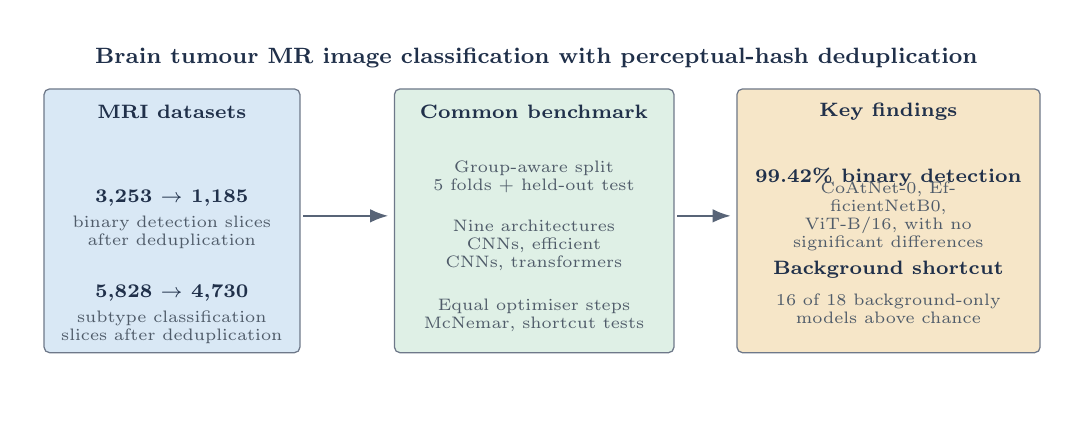
\begin{tikzpicture}[
  x=1cm,
  y=1cm,
  font=\sffamily,
  >=Latex,
  panel/.style={draw=nsnavy!65, fill=#1, rounded corners=2pt, line width=0.45pt},
  title/.style={font=\bfseries\fontsize{8.2}{9.0}\selectfont, text=nsnavy, align=center},
  heading/.style={font=\bfseries\fontsize{7.3}{8.1}\selectfont, text=nsnavy, align=center},
  body/.style={font=\fontsize{5.8}{6.5}\selectfont, text=nsmuted, align=center, text width=3.0cm},
  metric/.style={font=\bfseries\fontsize{7.0}{7.8}\selectfont, text=nsnavy, align=center},
  arrow/.style={->, line width=0.8pt, draw=nsnavy!75}
]
\fill[white] (0,0) rectangle (12.92,4.95);
\node[title, anchor=north] at (6.46,4.82)
  {Brain tumour MR image classification with perceptual-hash deduplication};

\node[panel=nsblue, minimum width=3.25cm, minimum height=3.35cm, anchor=north west] (data) at (0.20,4.18) {};
\node[heading] at (1.83,3.88) {MRI datasets};
\node[metric] at (1.83,2.78) {3,253 $\rightarrow$ 1,185};
\node[body] at (1.83,2.35) {binary detection slices\\after deduplication};
\node[metric] at (1.83,1.58) {5,828 $\rightarrow$ 4,730};
\node[body] at (1.83,1.15) {subtype classification\\slices after deduplication};

\node[panel=nsgreen, minimum width=3.55cm, minimum height=3.35cm, anchor=north west] (models) at (4.65,4.18) {};
\node[heading] at (6.43,3.88) {Common benchmark};
\node[body] at (6.43,3.05) {Group-aware split\\5 folds + held-out test};
\node[body] at (6.43,2.18) {Nine architectures\\CNNs, efficient CNNs, transformers};
\node[body] at (6.43,1.30) {Equal optimiser steps\\McNemar, shortcut tests};

\node[panel=nsamber, minimum width=3.85cm, minimum height=3.35cm, anchor=north west] (results) at (9.00,4.18) {};
\node[heading] at (10.93,3.88) {Key findings};
\node[metric] at (10.93,3.05) {99.42\% binary detection};
\node[body] at (10.93,2.55) {CoAtNet-0, EfficientNetB0,\\ViT-B/16, with no\\significant differences};
\node[metric] at (10.93,1.88) {Background shortcut};
\node[body] at (10.93,1.38) {16 of 18 background-only\\models above chance};

\draw[arrow] (3.50,2.56) -- (4.58,2.56);
\draw[arrow] (8.25,2.56) -- (8.93,2.56);
\end{tikzpicture}
\end{document}
